\chapter{Utviklingsprossesen}
\label{chap:process}


\section{Utviklingsmodell}
Oppdragsgiver uttrykte et ønske om tett oppfølging og innsikt underveis i prosjektet og god dokumentasjon for fremtidig vedlikeholdsarbeid. Det var også mulighet for endring eller tillegg av funksjoner i programvaren, så en smidig tilnærming var naturlig. \\ \\
På grunn av kravet til dokumentasjon tenkte vi raskt på Scrum som en god løsning og gruppen var allerede godt kjent med denne modellen. Vi undersøkte en del andre utviklingsmodeller, der Kanban og RUP kom frem som gode alternativ. Kanban er litt for løst strukturert for såpass uerfarne utviklere, siden det ikke er noen tidskrav for når hver funksjonalitet skal være ferdig. RUP er svært komplekst og ville ført til mye lengre planleggingstid om vi skal implementere den best mulig, siden vi ikke har noen erfaring med denne modellen.\\ \\ 
Under undersøkelsene kom vi over flere elementer fra andre utviklingsmodeller som ville være fordelaktige å implementere i vårt prosjekt. FDD har gode rutiner for å identifisere funksjonaliteter som legges til i backlogen\cite{FDD}. XP har mange gode verktøy for å standarisere koden og vi vil også implementere parprograming i størst mulig grad. Hvis en av oss ikke er i stand til å møte, eller et medlem jobber mer enn planlagt, vil vi gå gjennom endringene så fort vi har mulighet til å møtest. \\ \\
I implementasjonen vår av scrum vil Erland Ørbekk og Nils Kubberud fra Nammo ha rollen som Product Owners og Martin vil ha rollen som Scrum Master. Fordi vi ønsker å være selvorganiserende og lære mest mulig om estimering, vil Scrum Master ta på seg en del av ansvaret til Product Owners. Dersom Product Owners har noe spesifikt som de ønsker å prioritere vil det bli prioritert, men de har uttrykt et ønske om en mer veiledende enn bestemmende rolle i prosjektet. \\ \\
Vi valgte å ikke bruke alle elementene fra Scrum, vi valgte i stedet å bare plukke ut elementer som passet oss best. Elementer som daglige møter ble ikke holdt fordi vi hadde god kontroll over hva den andre jobbet med. Vi jobbet tett sammen som gjorde at vi hadde kontroll over hvor mye som hadde blitt gjort. Vi følte derfor at det ble veldig kunstig å ha et møte der vi diskutere progresjon, ettersom vi hadde full kontroll over motpartens arbeid.\\ \\
Vi brukte sprint elementene fra Scrum, vi satte opp møter med Nammo på slutten av hver sprint hvor vi forklarte hva som hadde blitt gjort denne sprinten. Vi klarte ikke å holde sprintene som vi hadde ønsket. Vi hadde problemer med feil estimering som gjorde at vi forandret sprintene. Vi jobbet videre med oppgavene vi hadde blitt utdelt, men oppgavene tok lengre tid enn estimert, det endte med at vi gikk bort fra sprinten.\\ \\
Vi brukte planing poker, men vi merket tidlig at vi fikk veldig lite fra tiden vi brukte. Vi klarte ikke estimere oppgavene,  og følte at hele prosessen var bortkastet tid vi heller skulle brukt på utvikling av programvare.\\ \\
Vi var veldig fornøyd med Srcum sin arbeidsmetode som jobbet på grunnleggende funksjonalitet som så bygges på videre, noe som er et kjerneelement i utviklingsmodellen.\\ \\


\section{Møter}

Møtene med Nammo valgte vi å sette opp litt etter vi hadde behov for dem, men vi prøvde å ta en tur til kontorene hver andre uke. dette ble satt opp litt etter behov, når vi hadde noen spørsmål som ikke lett kunne besvares på mail. Møtene ble i tillegg satt opp ettersom vi hadde noe å vise frem, en demo versjon for eksempel. Vi viste aldri Nammo noen direkt kode, men vi forklarte hva som hadde blitt gjort teoretisk så de kunne på bedre innsikt i hva som hadde blitt gjort. Det var lett å forklare teorien bak programmet ettersom Nils og Erland har en enorm mengde kunnskap i feltet sitt i tillegg gode kunnskaper i geometri og matematikk.\\
\\Et typisk møte på kontorene til Nammo på Raufoss, varierer på hvilket stadium i prosessen vi er. tidlig i prosessen brukte vi mye tid på hvilket verktøy vi skulle bruke, og hvilket som jobbet godt sammen. Når vi kommet lengre ut i utviklingsfasen, brukte vi møtene på spørsmål og uklarheter. Når vi hadde fått svar på det vi lurte på, forklarte vi hva som hadde blitt gjort og eventuelt vist en liten demo av hvordan ting virker. Dette ga Nammo en god oversikt over hvordan jobbingen gikk. Det var de fornøyd med og var mer interessert i noe som var gjort bygd fra bunnen så det kunne videreutvikles.

\subsection{Møte med veileder}
vi satt opp faste møter med Ivar hver tirsdag kl 13:00, disse møtene har hjulpet oss med å holde oss på rett spor. Møtene var avslappet og det var lett å komme med spørsmål og teorier. vi ble ofte sittende å tenke høyt på de største problemene. VI fikk mye ut av møtene, de var i tillegg lette å avlyse hvis det ikke var behov for dem eller det vare noe som krasjet. Etter å ha avlyst noen møter for bare å fortsette å jobbe når vi ikke hadde spørsmål. fant vi ut at det ikke var så lurt ettersom at vi hadde feiltolket oppgaven, merket vi at det er nyttig å ha møte bare for å passe på at vi holder oss på riktig spor.

\subsection{Gruppe møter} 
Vi avtalte å møte på skolen hver dag å jobbe, ettersom vi bare er to studenter på gruppen var det lett å møtes og jobbe sammen. vi jobbet tett i starten, med mye pairprogramming. Dette var nyttig, å jobbe sammen når vi begynte på et prosjekt som var ukjent for oss med et nytt programmeringsspråk. Når vi kom lengre ut i utviklingsprosessen ble vi jobbene mer hver for oss.


\section{Verktøy}
\subsection{Versjons kontroll}
Vi bestemte oss tidlig om hvilken versjonskontroll vi skulle bruke, det var egentilg ikke en avslutting men noe vi begge visste vi skulle bruke før vi begynte på prosjektet. Gjennom skolen gangen har vi brukt git siden andre semester. Når vi skulle ta for oss tema om versjonskontroll var vi begge enige om å bruke git. Git er den eneste versjonkontrollen noen av oss har brukt, så velge et nytt verktøy vi ikke har erfaring med virket ulogisk og tungvint. \\ \\
Vi valgte å hoste git repositoriet hos bitbucket, igjen fordi dette er det vi er vant til. Vi har såvidt prøvd github, men når vi satt opp repositoriet var det en vanesak å gå rett til bitbucket.
\subsection{Tekst editor}
Vi startet med å bruke Google docs som vår tekst editor. Vi valgte å jobbe på denne plattformen fordi vi ville ha en plattform vi kunne lett dele det som hadde blitt skrevet. Google Doc er i tillegg lett å ta i bruk det er ingen læringskurve i forhold til andre programmer som Latex. VI hadde originalt planlagt å bruke shareLatex som vår tekst editor. Vi hadde valgt å bruke denne løsningen fordi den ga oss muligheten til å dele dokumentet i tillegg til alle fordelene med Latex. Vi merket tidlig at en slik oppgave ikke passet i Google Docs, det var upraktisk og tregt å jobbe med store dokumenter i Google doc. Vi brukte da et dokument for hvert kapittel som var tungvint. Vi endte med å skrive de forskjellige kapitlene i hvert sitt Google Docs dokument for så å legge de inn i Latex. Vi valgte å gjøre det på denne måte fordi Latex gir et mye bedre slutt resultat enn Google Docs, men vi valgte å gjøre mesteparten av skrivingen i Google Docs fordi vi kunne lett skrive et utkast uten tanke på struktur. 

\subsection{IDE}
Når vi startet dette prosjektet viste vi ikke hvilken plattform vi skulle jobbe i. Det eneste vi hadde bestemt oss for var at vi skulle skrive programvaren i Python. Python var et språk ingen av oss hadde jobbet med før så vi hadde ingen preferanser. Vi endte opp med å bruke Eclipse sin utvidelse PyDev. Vi valgte å bruke denne plattformen fordi den var godt anbefalt i av Python miljøet i tillegg til at vi hadde begge en liten kjennskap til Eclipse. \\ \\
Vi trengte en måte å gjøre programvaren brukervennlig. Vi valgte derfor å ta i bruk Tkinter fordi det kom godt anbefalt i tillegg til at var kompatibelt med MatPlotLib. Vi så kort på qt som en mulighet for utvikling av GUI, men vi endte med Tkinter. Noe vi ikke var helt fornøyd med i ettertid på grunn av vanskeligheter til å plassere grafene på riktig plass. Vi fikk inn grafen fra MatPlotLib uten problemer, men etterhvert som vi implementert flere inputfelt og grafer  fikk vi ikke ting der vi ville. Vi valgte å bruke MatPlotLib for å viste brukeren hvordan stjerneformen han valgte ville bli seendes ut. 
\section{Problemer vi har møtt under utviklingsprosessen}


\subsection{Problemer med clicklistener og MVC}
Vi møtte tidlig på et problem med arkitektur modellen når vi skulle implementere visnings delen. Vi bruker her en clickListner() funksjon som konstant ser om en knapp har blitt trykket. Dette bruker vi vår brukeren oppgir parametere for rakettmotoren. I vår første prototype hadde vi ikke implementert en arkitekturmodell, vi kjøret hovedprogrammet for visnings filen. Når vi skulle implementere MVC møtte vi på en utfordring ettersom alle logiske beregninger skulle foregå i en annen mappe. Vi kunne ikke lengre bruke visnings modellen til å kjøre programmet å måtte finne en løsning på hvordan vi skulle kjøre programvaren. Løsningen vår var å lage en egen fil som kun håndtere overgangen mellom modellene. Denne inneholder syv funksjoner som gjør oppdaterer variablene og gjør det mulig for oss å bruke MVC.


\subsection{Minnekapasitet}
Et problem vi møtte på tidlig var størrelsen på arrayen vår. Med Nammo sitt krav på høy nøyaktighet måtte vi ha en enorm mengde punkter. Dette ville gi problemer i 2D, men spesielt for videre utvikling til 3D. I oppgaven vår skulle vi lage en solid 2D versjon som kan bygges videre på. Vi kunne se dette ville bli et problem når programvaren skal kjøres på en vanlig arbeids laptop.\\ \\
Vi tok problemet til veilederen der vi diskuterte problemet, etter en god stund kom vi frem til at hvis formen som skal skjæres ut er symmetrisk trenger vi ikke beregne hele formen, men i stedet bare en liten bit. Denne biten kunne da speiles, for en presentasjon. Vi kontaktet Nammo, som verifiserte at alle stjerneformede var symmetriske. Dette betyr at vi kan beregne en liten “kakebit” som kutter minneforbruket enormt. Vi så her at vi kunne dele opp formen på hver arm av stjernen. Så vi deler en arm i to biter, dette gjør at jo flere armer stjernen har, jo mindre er minneforbruket.



\subsection{Implisit vs Eksplisit}
Det største problemet vi møtte under denne oppgaven var desidert kollapsende vegger. Når en stjerneform brenner vil armene etterhvert krasje inn i hverandre og kollapse sammen. Dette skaper et stort problem for koden, fordi det er veldig vanskelig å vite om to punkter har krasjet eller om de holder på å kræsje. Vi har satt opp algoritmen så vi har en array med en rekke punkter, vi har ingen kontroll hvor de er i forhold til hverandre. Dette er det største problemet med eksplisitt løsning. Vi kunne gå over til en implisitt løsning som ville løst dette problemet, men det betydde at vi måtte begynne helt på nytt. i tillegg kommer en implisitt med en hel rekke nye problemer. \\ \\
En implisitt løsning betyr at vi har en flate dekket med punkter som er satt til 0. Når brennflaten vokser forflytter den som over punktene og når den passerer et punkt, blir det satt til 1. ( trenger bilde som forklarer ) Det største problemet med denne er minneforbruket. Det hadde vært en god løsning hvis nøyaktighet hadde vært så viktig. Med Nammo sitt høye krav på nøyaktighet ville dette gi store problemer. Vi måtte bruke en enorm mengde punkter for at algoritmen skulle bli nøyaktig nok. Vi valgte derfor å holde oss til en eksplisitt løsning.\\ \\
Måten vi valgte å løse dette problemet på var ved å bruke løsningen på minneforbruket. når vi delte opp formen laget vi en symmetrilinje. Vi vet at formen er symmetrisk dette gjør at vi kan håndtere de kollapsede veggene. Før hadde vi ikke kontroll over hvilke punkter som krysset hverandre. Dette gjorde at vi ikke ville klare å håndtere når veggene kollapset sammen. Når vi tar og deler stjerne armen på langs vet vi at den er identisk på den andre siden.\\ \\



\begin{figure}[h]
    \centering
    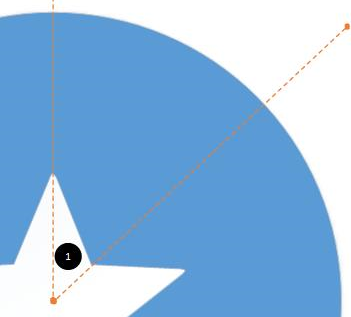
\includegraphics[width=\textwidth]{pngstjerne}
    \caption{Ilustrasjon av symemetrilinjen}
    \label{fig:my_label}
\end{figure}



\subsection{Symmetrilinjen}
kanskje skrive mer \\ \\
\clearpage

\subsection{Punkt forflytting vs linje forflytting} 
Vi møtte på et uforventet problem med forflytningen når vi begynte å nærme oss en ferdig prototype. Vi merket et problem rundt indre hjørner, et indrehjørne et hjørne som forflytter seg innover og holder sin vinkel, i motsetning til et ytrehjørne som vokser utover og får en mindre vinkel for hvert steg. \\
\begin{figure}[h]
    \centering
    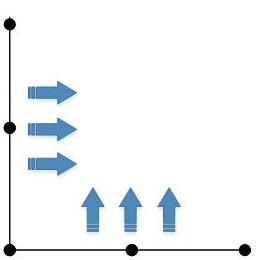
\includegraphics[width=0.5\textwidth]{nyindre}
    \caption{Ilustrasjon av indre hjørne}
    \label{fig:my_label}
\end{figure}

\noindent
Vi merket at det indre hjørnet ikke beholde vinkelen sin som den skal. Med vår punktvis forflytning, flytter alle punkter seg like langt. Dette skaper problemer i et indre hjørne, i et indre hjørne skal hjørne punktet flytte seg lengre enn de andre punktene for å beholde vinkelen sin. Med vår punktvis forflytning endte det med at hjørne punktet ble hengende igjen å lage en skarpere vinkel for hvert steg. For å løse dette problemet måtte vi endre den grunnleggende algoritmen i forflytningen.\\ 
\begin{figure}[h]
    \centering
    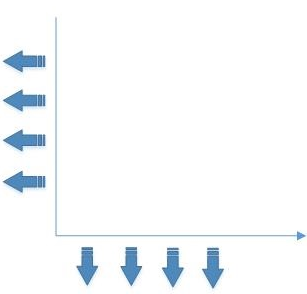
\includegraphics[width=0.5\textwidth]{nyytre}
    \caption{Ilustrasjon av ytre hjørne}
    \label{fig:my_label}
\end{figure}
\clearpage
\noindent
Vi valgte å løse dette problemet med å skrive om den punktvise forflytningen til en versjon som flyttet linjestykkene i stedet for punktene. Som vist øverst til venstre på figur \ref{fig:sloyfe} flytter vi hele linjestykket i stedet for punktene. Dette løser problemet med indre hjørner. Vi flytter hele linjen og når de krysser hverandre kan vi finne krysningspunktet på linjene og legge det nye punktet der. Da vil det indre hjørnet beholde vinkelen sin for hvert steg. \\ \\
\begin{figure}[h]
    \centering
    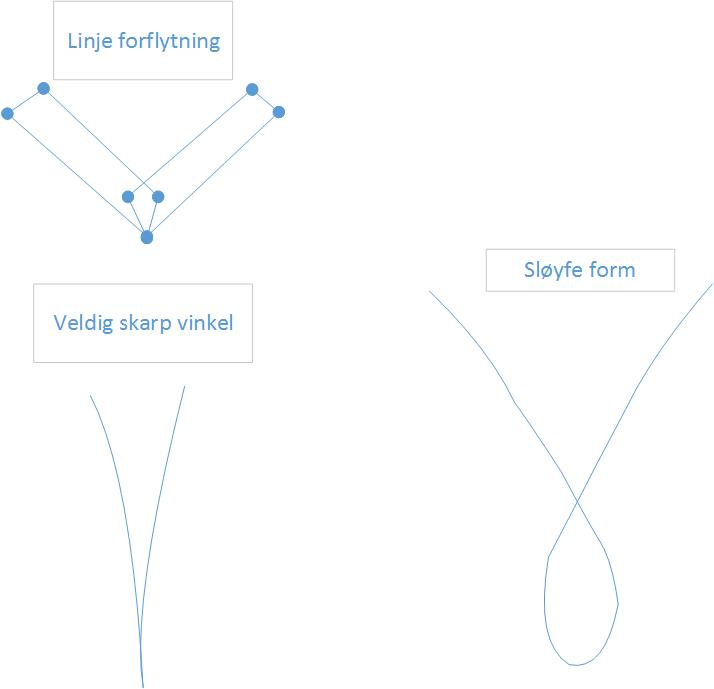
\includegraphics[width=0.5\textwidth]{pngSloyfeform}
    \caption{Ilustrasjon av linjeforflytning og sløyfeform}
    \label{fig:sloyfe}
\end{figure}

\noindent
Denne løsningen kom også med sine ulemper. Når et ytre hjørne forflytter seg minsker vinkelen dens, dette gjør at vi vil få tomrom mellom linjene våre. Så vi må legge på et lite linjestykke mellom hvert linjestykke i det ytre hjørne. Dette gjør at vi vil ha en eksponentiell økning av linjestykker i ytre hjørner. Vi måtte derfor modifisere algoritmen så den slår sammen linjestykker under en viss lengde for å minimere minneforbruket.\\ \\
Denne løsningen komme med flere potensielle problemer. Hvis algoritmen møter en veldig skarp vinkel kan linjestykkene flytte seg for langt. Dette gjør at algoritmen ikke oppdager at den har krysset sin nabo og vil fortsette å vokse å lage en slags sløyfe form. Dette er veldig usannsynlig hendelse, men vi valgte å ta hensyn til den for å gjøre algoritmen så robust som mulig.\\ \\
Måten vi løste dette på var ved å kjøre en for loop for hvert linjestykke i arrayen. Vi tar det linjestykke og sjekker om det krysser et annet linjestykke i arrayen. Hvis det krysser et annet linjestykke enn det ved siden av seg har det begynt på en sløyfeform.  

 





